\section{W3: Scheduling, Memory Management}
\textbf{Why multiprogramming?} better CPU utilization, allows I/O overlap, better responsiveness of computer.\\
\textbf{Preemption:} Preemptive scheduling is when the scheduler decides to switch to another process/thread. Clock interrupts used upon a quantum. Non-preemptive scheduling is when the process/thread itself decides to give up the CPU or is blocked.\\
\textbf{Context switch:} Switching from one process/thread to another is expensive.\\

\subsection{Non-preemptive scheduling}
\textbf{First-come, first-served (FCFS):} Simple, but long average waiting time.\\
\textbf{Shortest job first (SJF):} Shortest average waiting time, but long waiting time for long processes/threads. Average turnaround time is minimized.\\

\subsection{Preemptive scheduling}
\textbf{Round-robin (RR):} Each process/thread gets a quantum.\\
\textbf{Shortest remaining time first (SRTF):} Shortest average waiting time, but long waiting time for long processes/threads. Average turnaround time is minimized.\\
\textbf{Priority scheduling:} Each process/thread has a priority. May lead to starvation.\\

\subsection{Memory management}
\textbf{Why Memory Management?} Support multiprogramming. Secure isolation between processes/threads and OS memory. Enables virtual memory which allows processes/threads to use more memory than is physically available.\\
\textbf{No memory abstraction:} Use swap space on disk. Multiplex physical memory.\\

\subsubsection{Memory abstraction}
\textbf{Logical address space:} set of addresses that a process/thread can use which are mapped to physical addresses.\\
\textbf{Base and limit registers:} base register holds start address of process/thread, limit register holds size of process/thread.\\
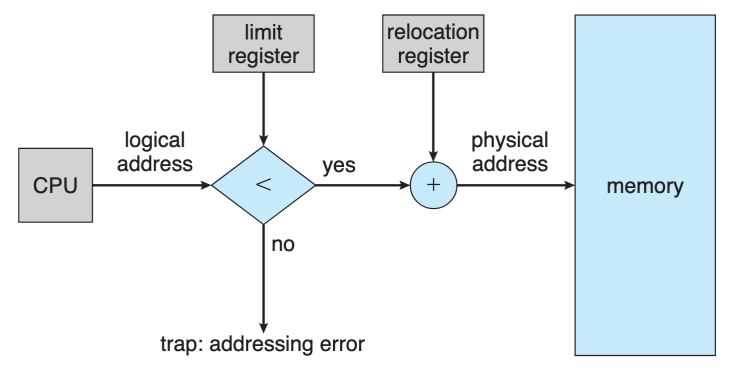
\includegraphics[width=\linewidth]{figs/base-and-limit-registers.png}
\textbf{Memory management unit (MMU):} hardware device that maps logical addresses to physical addresses.\\
\textbf{Manage free memory:} using bitmap or linked list.\\
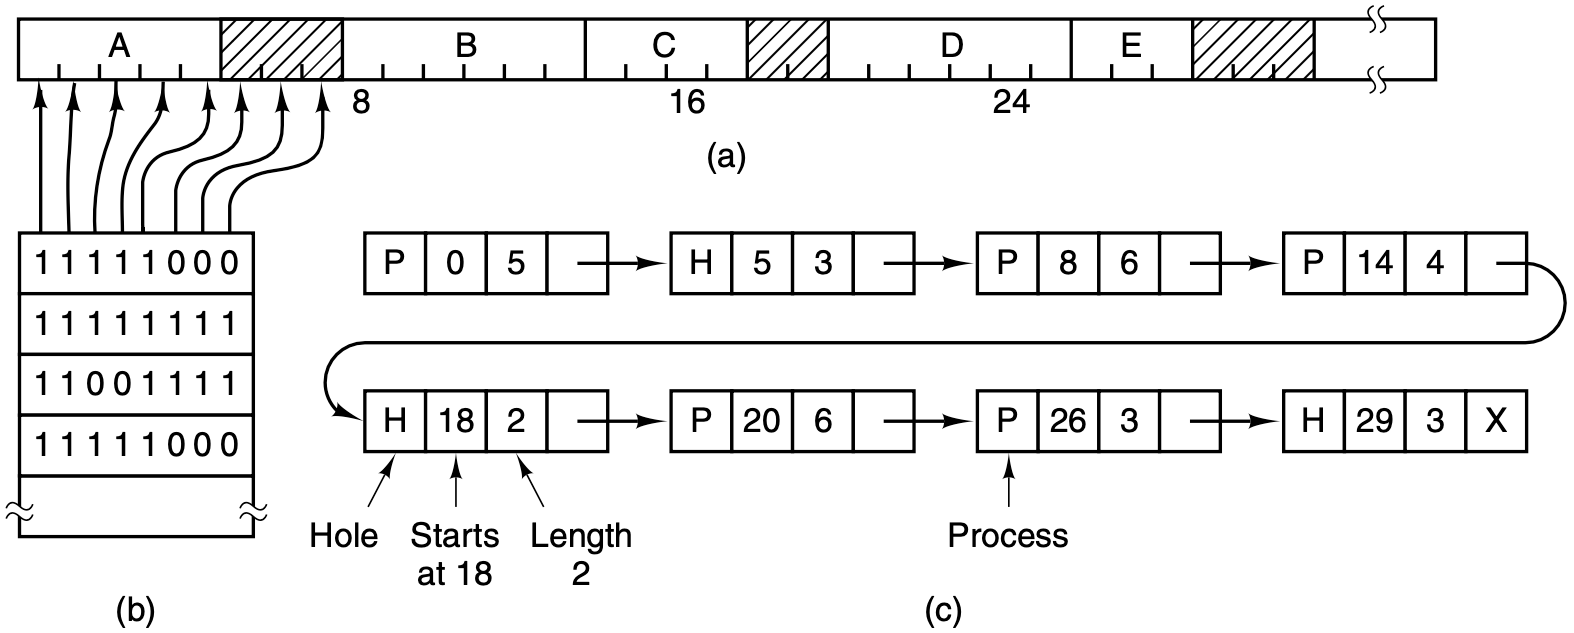
\includegraphics[width=\linewidth]{figs/memory-management.png}
\textbf{Why virtual memory?} Processes/threads can use more memory than is physically available.\\
\textbf{Page table:} maps virtual pages to physical pages.\\
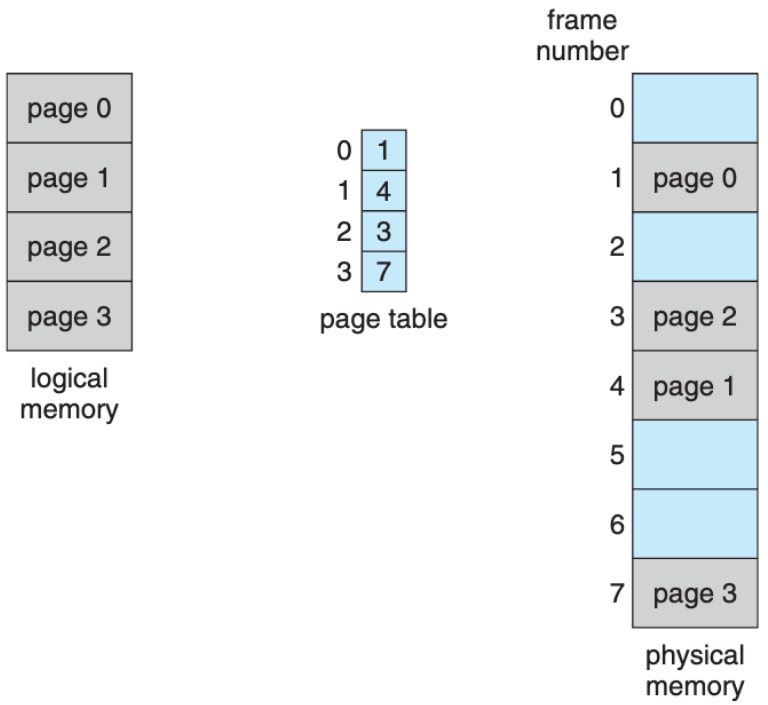
\includegraphics[width=0.6\linewidth]{figs/paging-model.png}\\
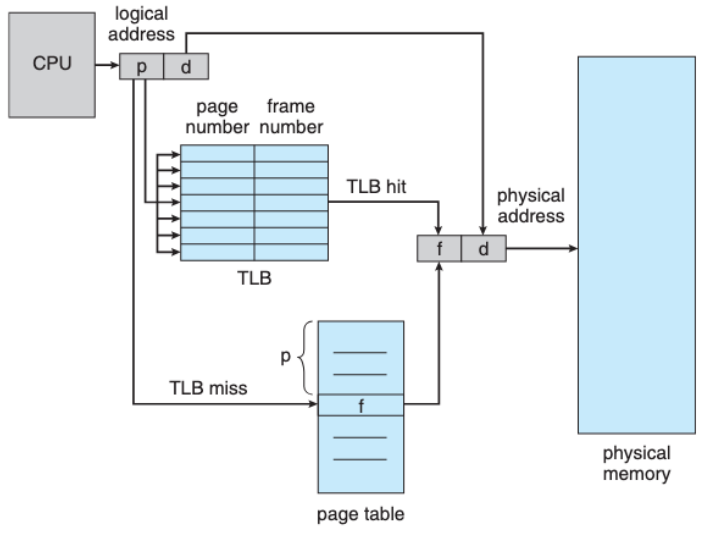
\includegraphics[width=\linewidth]{figs/mmu-with-tlb.png}\\
\textbf{Translation Lookaside Buffer (TLB):} cache for page table, faster than main memory, speeds up address translation.\\
\textbf{Page replacement algorithms for TLB:} \textit{NRU} (Not Recently Used, R and M bit, 4 classes creating combination of referenced and in highest priority order of R'M', R'M, RM', RM).\\
